\documentclass[tikz,border=6pt]{standalone}
\usepackage[utf8]{inputenc}
\usepackage[T1]{fontenc}
\usepackage{amsmath}
\usetikzlibrary{arrows.meta}

\begin{document}
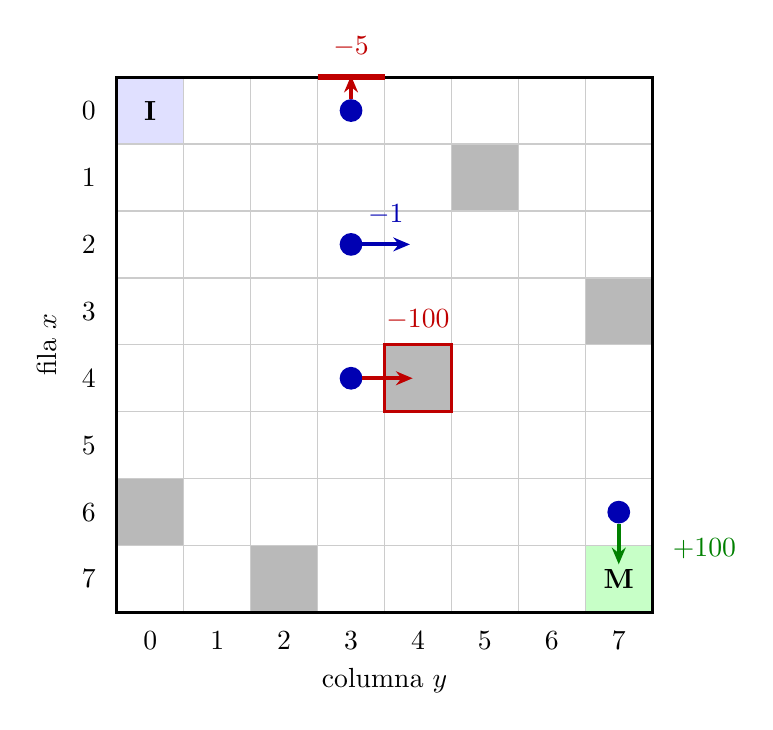
\begin{tikzpicture}[scale=0.85]
    \fill[blue!12] (0, 7) rectangle (1, 8);
    \node[font=\bfseries] at (0.5, 7.5) {I};

    \fill[green!22] (7, 0) rectangle (8, 1);
    \node[font=\bfseries] at (7.5, 0.5) {M};

    \foreach \r/\c in {1/5, 3/7, 4/4, 6/0, 7/2} {
        \fill[gray!55] (\c, 7-\r) rectangle (\c+1, 8-\r);
    }

    \draw[gray!40, line width=0.5pt] (0, 0) grid (8, 8);
    \draw[black, line width=1.1pt] (0, 0) rectangle (8, 8);

    \foreach \i in {0,...,7} {
        \node at (-0.42, 7.5-\i) {\i};
        \node at (\i+0.5, -0.42) {\i};
    }
    \node[rotate=90] at (-1.05, 4.0) {fila $x$};
    \node at (4.0, -1.02) {columna $y$};

    % Wall hit (-5) at (0,3) facing North
    \draw[red!75!black, line width=2.2pt] (3, 8) -- (4, 8);
    \fill[blue!70!black] (3.5, 7.5) circle (0.17);
    \draw[-{Stealth[length=6pt, width=5pt]}, red!75!black, line width=1.5pt] (3.5, 7.67) -- (3.5, 8.02);
    \node[red!75!black] at (3.5, 8.45) {$-5$};

    % Regular step (-1) from (2,3) to (2,4)
    \fill[blue!70!black] (3.5, 5.5) circle (0.17);
    \draw[-{Stealth[length=6pt, width=5pt]}, blue!70!black, line width=1.5pt] (3.67, 5.5) -- (4.38, 5.5);
    \node[blue!70!black] at (4.02, 5.95) {$-1$};

    % Collision with obstacle (-100) from (4,3) into obstacle at (4,4)
    \draw[red!75!black, line width=1.2pt] (4, 3) rectangle (5, 4);
    \fill[blue!70!black] (3.5, 3.5) circle (0.17);
    \draw[-{Stealth[length=6pt, width=5pt]}, red!75!black, line width=1.5pt] (3.67, 3.5) -- (4.42, 3.5);
    \node[red!75!black] at (4.5, 4.38) {$-100$};

    % Goal (+100) from (6,7) into (7,7)
    \fill[blue!70!black] (7.5, 1.5) circle (0.17);
    \draw[-{Stealth[length=6pt, width=5pt]}, green!50!black, line width=1.5pt] (7.5, 1.33) -- (7.5, 0.72);
    \node[green!50!black] at (8.78, 0.95) {$+100$};
\end{tikzpicture}
\end{document}
